\section{Введение}

Измерения физических величин всегда содержат некоторое отклонение от истинного значения, так как не существует абсолютно точных приборов и методов, поэтому важно оценивать степень точности.

Существуют разные виды погрешностей: одни возникают из-за случайных изменений условий эксперимента, другие обусловлены особенностями используемого оборудования и методик, а третьи связаны с ошибками оператора. Чтобы уменьшить влияние таких отклонений, измерения проводят многократно, получая серию значений, которые затем анализируются.

Оценка погрешности является неотъемлемой частью любого эксперимента, так как позволяет повысить точность получаемых данных и сделать выводы более обоснованными. Корректный учёт возможных ошибок в измерениях обеспечивает надёжность полученных результатов и их применимость в научных и технических исследованиях.

\subsection{Решаемые задачи}

\begin{enumerate}
    \item Освоить методику использования измерительного прибора для многократного прямого измерения физической величины.
    \item Выполнить простейшую статистическую обработку серии результатов наблюдений  при прямых измерениях.
\end{enumerate}

\section{Основная часть}

\subsection{Теоретическая часть}

При проведении физических измерений невозможно получить экспериментальные данные без отклонения от истинного значения. Погрешности измерений бывают:
\begin{itemize}
    \item Систематические, которые возникают из-за несовершенства метода измерений или калибровки прибора. Они проявляются одинаково при каждом измерении.
    \item Случайные, возникающие из-за случайных факторов и не имеющие определённого направления, их можно уменьшить за счет многократных измерений.
    \item Грубые (промахи), которые возникают из-за ошибок экспериментатора и должны исключаться при обработке данных.
\end{itemize}

Обычно общее значение записывается в виде:
\begin{equation}
    X=X_{изм}\pm \Delta X
\end{equation}
где $X_{изм}$ -- полученное экспериментальное значение, а $\Delta X$ -- приближенная погрешность измерения. Но на самом деле утверждать можно только то, что $X$ попадает в этот диапазон только с какой-то вероятностью, и она тем выше, чем точнее проведены измерения.

При многократных измерениях получают серию значений, которая называется выборкой:
\begin{equation}
    x_1,x_2,x_3, ..., x_n
\end{equation}

Для уменьшения влияния случайных погрешностей проводят серию измерений и вычисляют среднее арифметическое:
\begin{equation}
    \overline{x}=\frac{x_1+x_2+...+x_n}{n}=\frac{1}{n}\sum_{i=1}^{n} x_i
\end{equation}
где $n$ -- количество измерений, $x_i$ -- отдельные результаты измерений. Чем больше измерений проведено, тем точнее будет полученное среднее значение.

Дисперсия (средняя квадратичная погрешность отдельного наблюдения) оценивается по формуле:
\begin{equation}
\label{eq:3}
    \sigma=\sqrt{\frac{1}{n-1}\sum_{i=1} (x_i-\overline{x})^2}
\end{equation}

Средняя квадратичная погрешность среднего определяется как:
\begin{equation}
\label{eq:4}
    \sigma_{\overline{x}}=\frac{\sigma}{\sqrt{n}} ,
\end{equation}
Это означает, что увеличение числа измерений помогает уточнить значение величины и уменьшить интервал, в котором с определённой вероятностью лежит значение $X$. Он задаётся как:
\begin{equation}
    x=\overline{x}\pm\sigma_{\overline{x}} ,
\end{equation}

\subsection{Эксперимент}
Блок-схема установки приведена на рис.~\ref{fig:Scheme}. На рис.~\ref{fig:photo1} и рис.~\ref{fig:photo2} представлены частотомер и генератор импульсов.

Генератор сигналов передаёт на частотомер последовательность прямоугольных импульсов с заданными параметрами. Частота измеряется на двух шкалах: грубой и точной. Для измерений используется генератор импульсов Г5-15 и частотомер Ч3-32.

\begin{figure}[ht!]
\centering
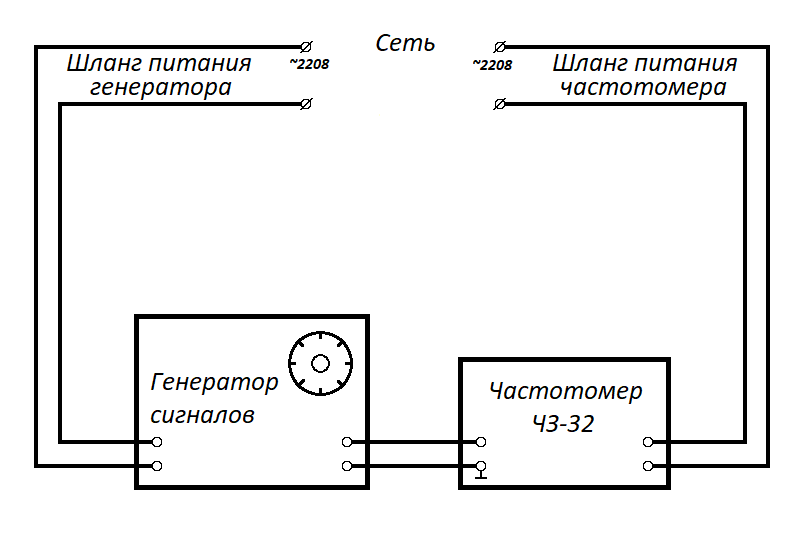
\includegraphics[width=0.9\textwidth]{Scheme.png}
\caption{Блок-схема установки для измерения частоты импульсов}
\label{fig:Scheme}
\end{figure}

\begin{figure}[ht!]
\centering
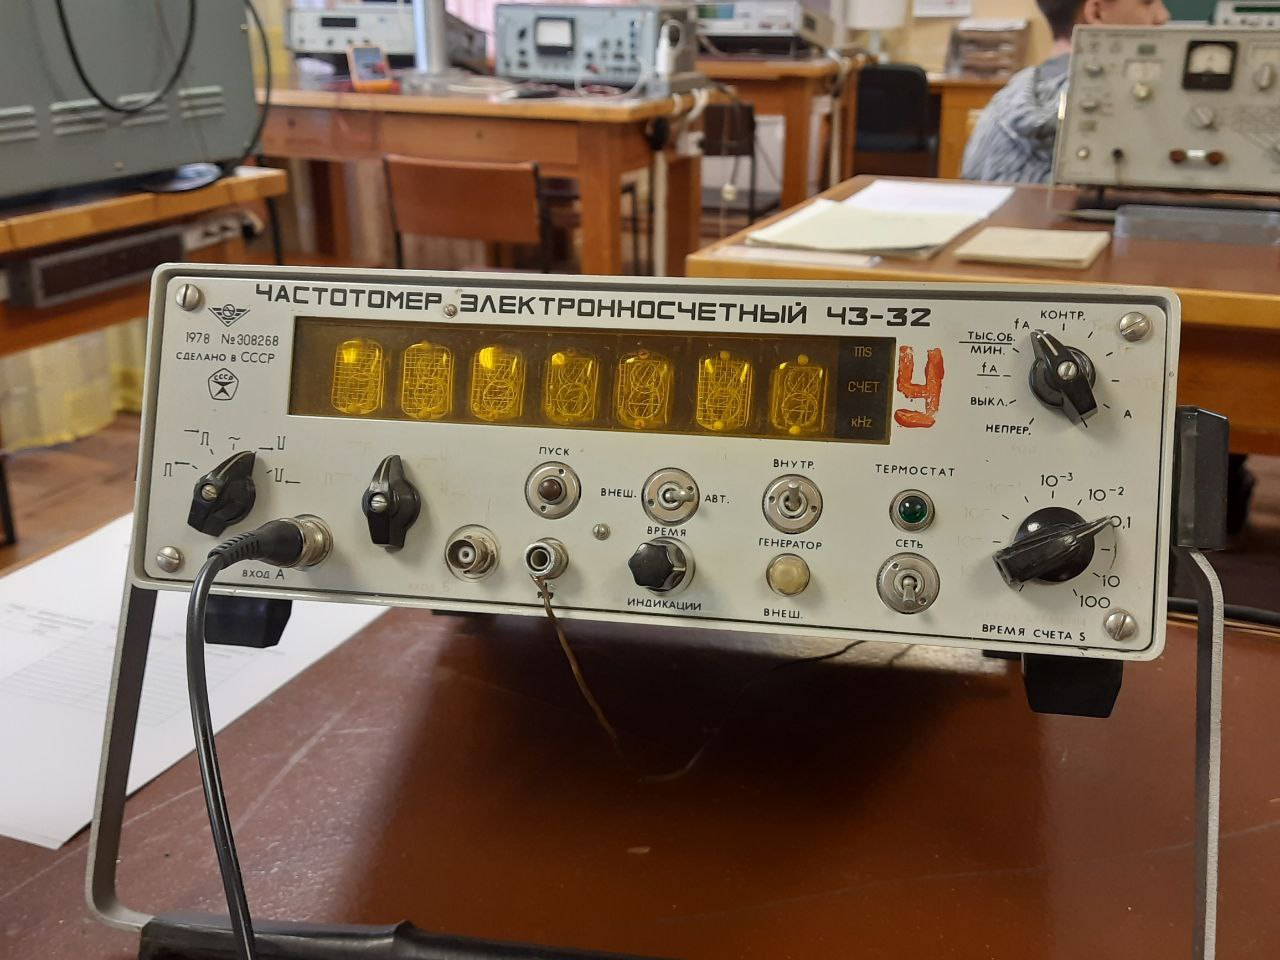
\includegraphics[width=0.8\textwidth]{photo1.jpg}
\caption{Фотография частотомера Ч3-32}
\label{fig:photo1}
\end{figure}

\begin{figure}[ht!]
\centering
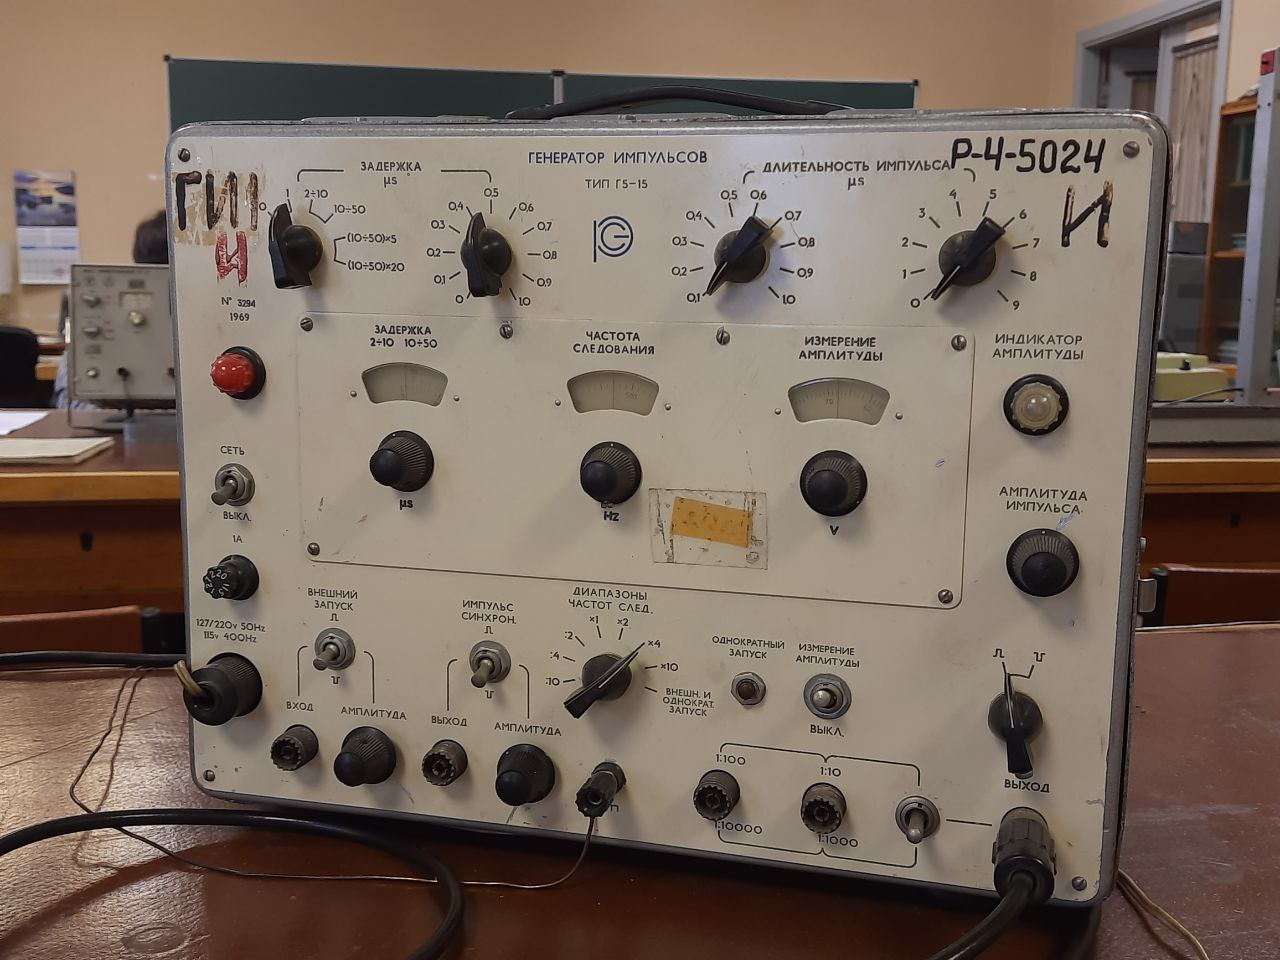
\includegraphics[width=0.8\textwidth]{photo2.jpg}
\caption{Фотография генератора импульсов}
\label{fig:photo2}
\end{figure}

\subsection{Обработка данных и обсуждение результатов}

Вычисление погрешности прибора:
\begin{equation}
\label{eq:1}
   \gamma_f=  \frac{\Delta_f}{\overline{f}} \cdot 100\%
\end{equation}
\begin{equation}
\label{eq:2}
 \gamma_f=\pm(\gamma_0+\frac{1}{(\overline{f} \cdot T)}) \cdot 100\%
 \end{equation}
 Где  $\gamma_0$  -- основная относительная погрешность частоты, $ \gamma_0 = \pm5 \cdot 10^{-7} $; $\overline{f}$ -- среднее значение всех измеряемых частот в кГц; $T$ -- время измерения в с, $T$ = 0,1 с. на грубой шкале, $T$ = 1 с. на точной шкале.
 
\subsubsection{Таблицы}

В таблице ~\ref{tabl:1} представлены результаты десяти измерений частоты на грубой шкале.

Было получено среднее значение измерений на грубой шкале: $\overline{f} = 4.56 $ гКц.

В ходе работы было проведено пятьдесят измерений частоты на точной шкале, однако несколько начальных значений допускали грубую погрешность и были убраны из рассмотрения и выборки. Таким образом, в таблице ~\ref{tabl:2} представлены результаты сорока трёх измерений частоты на точной шкале.

Для точной шкалы была высчитана погрешность прибора: $\Delta f = 0.001002$ кГц.

\begin{center}
\begin{table}
\centering
\caption{Измерения на грубой шкале}
\label{tabl:1}
\begin{tabular}{|c|c|c|c|c|}
\hline
\begin{minipage}{7mm}
    № п.п. 
\end{minipage}&
\begin{minipage}{5cm}
\begin{center}
    Диапазон показаний использованной шкалы прибора
\end{center}
\end{minipage} &
\begin{minipage}{5cm}
\begin{center}
    Результаты отдельных наблюдений
    
    ($f_i$)
\end{center}
\end{minipage} &
\begin{minipage}{5cm}
\begin{center}
    Погрешность прибора на данной шкале
    
    ($\Delta f_{приб}$)
\end{center}
\end{minipage}\\
\hline
{}&(кГц)&(кГц)&(кГц)\\
\hline
1 & 0-10^5  &  4.56  &  0.0100 \\
2 & 0-10^5  &  4.54  &  0.0100 \\
3 & 0-10^5  &  4.54  &  0.0100 \\
4 & 0-10^5  &  4.56  &  0.0100 \\
5 & 0-10^5  &  4.56  &  0.0100 \\
6  & 0-10^5  &  4.56  &  0.0100 \\
7  & 0-10^5  &  4.58  &  0.0100 \\
8  & 0-10^5  &  4.56  &  0.0100 \\
9  & 0-10^5  &  4.58  &  0.0100 \\
10 & 0-10^5  &  4.56  &  0.0100 \\
\hline
\end{tabular}
\end{table}
\end{center}

\begin{center}
\begin{table}[h!]
\centering
\caption{Результаты точных измерений}
\label{tabl:2}
\begin{tabular}{|c|c|c|c|c|}
\hline
\begin{minipage}{7mm}
    № п.п. 
\end{minipage}&
\begin{minipage}{5cm}
\begin{center}
    Результаты отдельных наблюдений 
    
    ($f_i$)
\end{center}
\end{minipage} &
\begin{minipage}{5cm}
\begin{center}
    Случайные отклонения от среднего
    
    ($d_i = f_i - \overline{f}$)
\end{center}
\end{minipage} &
\begin{minipage}{5cm}
\begin{center}
    ($d_i^2 = (f_i - \overline{f})^2$)
\end{center}
\end{minipage}\\
\hline
{}&(кГц)&(кГц)&(кГц^2)\\
\hline
1  &    4.542  &   0.001000  &  0.000001000 \\
2  &    4.540  &  -0.001000  &  0.000001000 \\
3  &	4.538  &  -0.003000  &  0.000009000 \\
4  &	4.542  &   0.001000  &  0.000001000 \\
5  &	4.542  &   0.001000  &  0.000001000 \\
6  &	4.542  &   0.001000  &  0.000001000 \\
7  &	4.540  &  -0.001000  &  0.000001000 \\
8  &	4.542  &   0.001000  &  0.000001000 \\
9  &    4.542  &   0.001000  &  0.000001000 \\
10 &	4.542  &   0.001000  &  0.000001000 \\
11 &	4.542  &   0.001000  &  0.000001000 \\
12 &	4.542  &   0.001000  &  0.000001000 \\
13 &	4.542  &   0.001000  &  0.000001000 \\
14 &	4.544  &   0.003000  &  0.000009000 \\
15 &	4.544  &   0.003000  &  0.000009000 \\
16 &	4.544  &   0.003000  &  0.000009000 \\
17 &	4.544  &   0.003000  &  0.000009000 \\
18 &	4.544  &   0.003000  &  0.000009000 \\
19 &	4.542  &   0.001000  &  0.000001000 \\
\hline
\end{tabular}
\end{table}
\end{center}

\begin{center}
\begin{tabular}{|c|c|c|c|c|}
\hline
\begin{minipage}{7mm}
    № п.п. 
\end{minipage}&
\begin{minipage}{5cm}
\begin{center}
    Результаты отдельных наблюдений 
    
    ($f_i$)
\end{center}
\end{minipage} &
\begin{minipage}{5cm}
\begin{center}
    Случайные отклонения от среднего
    
    ($d_i = f_i - \overline{f}$)
\end{center}
\end{minipage} &
\begin{minipage}{5cm}
\begin{center}
    ($d_i^2 = (f_i - \overline{f})^2$)
\end{center}
\end{minipage}\\
\hline
{}&(кГц)&(кГц)&(кГц^2)\\
\hline
20 &	4.542  &   0.001000  &  0.000001000 \\
21 &	4.540  &  -0.001000  &  0.000001000 \\
22 &	4.540  &  -0.001000  &  0.000001000 \\
23 &	4.542  &   0.001000  &  0.000001000 \\
24 &	4.540  &  -0.001000  &  0.000001000 \\
25 &	4.542  &   0.001000  &  0.000001000 \\
26 &	4.540  &  -0.001000  &  0.000001000 \\
27 &	4.540  &  -0.001000  &  0.000001000 \\
28 &	4.540  &  -0.001000  &  0.000001000 \\
29 &	4.538  &  -0.003000  &  0.000009000 \\
30 &	4.540  &  -0.001000  &  0.000001000 \\
31 &	4.540  &  -0.001000  &  0.000001000 \\
32 &	4.540  &  -0.001000  &  0.000001000 \\
33 &	4.540  &  -0.001000  &  0.000001000 \\
34 &	4.540  &  -0.001000  &  0.000001000 \\
35 &	4.538  &  -0.003000  &  0.000009000 \\
36 &	4.540  &  -0.001000  &  0.000001000 \\
37 &	4.538  &  -0.003000  &  0.000009000 \\
38 &	4.540  &  -0.001000  &  0.000001000 \\
39 &	4.538  &  -0.003000  &  0.000009000 \\
40 &	4.538  &  -0.003000  &  0.000009000 \\
41 &	4.538  &  -0.003000  &  0.000009000 \\
42 &	4.542  &   0.001000  &  0.000001000 \\
43 &	4.541  &   0         &  0           \\
\hline
   & $\overline{f}$=4.541 & $\sum_{i=1}^{50} d_i= -0.006000$ & $\sum_{i=1}^{50}d_i^2=0.0001380$\\
\hline
\end{tabular}
\end{center}

\begin{center}
\begin{table}[h!]
\centering
\caption{Таблица распределения}
\label{tabl:3}
\begin{tabular}{|c|c|c|c|c|}
\hline
\begin{minipage}{1cm}
    № п.п.
\end{minipage}&
\begin{minipage}{5cm}
\begin{center}
    Границы интервалов
\end{center}
\end{minipage} &
\begin{minipage}{5cm}
\begin{center}
    Количество попаданий результата в интервал

    ($\Delta n$)
\end{center}
\end{minipage} &
\begin{minipage}{5cm}
\begin{center}
    Доля полного числа результатов, попадающих в этот интервал
    
    ($\delta n=\frac{\Delta n}{n}$)
\end{center}
\end{minipage}\\
\hline
1 &  [4.538,4.540)  &  7   &  0.16  \\
2 &  [4.540,4.542)  &  16  &  0.37  \\
3 &  [4.542,4.544)  &  15  &  0.35  \\
4 &  [4.544,4.546)  &  5   &  0.12  \\
\hline
\end{tabular}
\end{table}
\end{center}

В ходе работы были высчитаны следующие величины:

Дисперсия: $\sigma=0.001813$ кГц.

Средняя квадратичная погрешность среднего: $\sigma_f=0.0002764$ кГц.

Случайная и системная погрешности имеют одинаковый порядок, поэтому можно применить следующую формулу суммарной погрешности:
\begin{equation}
\label{eq:5}
\sigma_{сумм}=\sqrt{(\frac{\Delta f}{3})^2+\sigma_f^2}
\end{equation}
Таким образом, суммарная погрешность: $\sigma_{сумм}=0,0004336$ кГц.

Окончательный ответ имеет вид: $f=4.541\pm0.0004336$ кГц.

\subsubsection{Описание программ}
Для проведения расчётов на языке $C++$ были написаны программы "Rough measure"\ и "Precise measure"\verb|,| предназначенные для обработки данных с грубой и точной шкал соответственно.

Программа "Rough measure"\ состоит из пяти функций: in (), fx(), rel(), abs() и out(). Первая функция отвечает за ввод данных из файла "Rough measuring.csv"\ в массив a. Функция fx() высчитывает среднее арифметическое значение из полученных данных массива a. Функции rel() и abs() рассчитывают относительную и абсолютную погрешности с использованием формул (\ref{eq:1}) и (\ref{eq:2}) соответственно. Функция out() выводит среднее арифметическое значение и абсолютную погрешность с округлением до четырёх значащих цифр в файл "Rough result.csv".

Программа "Precise measure"\ построена похожим образом и берет значения для обработки из файла "Precise measuring.csv"\ с помощью функции in (). Функции fx(), rel() и abs() работают аналогично функциям из программы для обработки грубых значений. Функции sygma() и sygma\_x() по формулам (\ref{eq:3}) и (\ref{eq:4}) соответственно высчитывают значения средней квадратичной погрешности отдельного наблюдения и средней квадратичной погрешности среднего. sum\_err() по формуле (\ref{eq:5}) высчитывает значение суммарной погрешности. Функция columns() принимает массивы b и c и записывает в них значения $d_i$ и $d_i^2$ для второй и третьей колонок в таблице для точных измерений. Последняя функция out() выводит значения среднего арифметического, абсолютной погрешности, дисперсии, средней квадратичной погрешности среднего, суммарной погрешности, результаты вычислений столбцов значений $d_i$ и $d_i^2$ для разных измерений и их сумм в файл "Precise result.csv".


\subsubsection{Графики}

На рис.~\ref{fig:plot1}, рис.~\ref{fig:plot2}, рис.~\ref{fig:plot3}, рис.~\ref{fig:plot4} приведены результаты работы программы gnuplot.

\begin{figure}
\centering
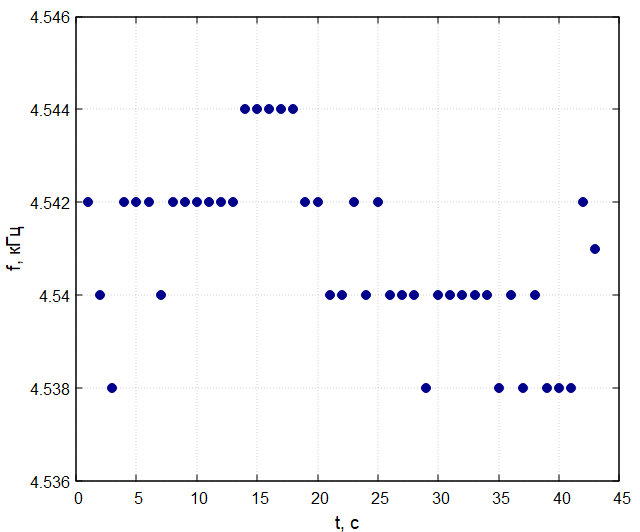
\includegraphics[width=0.8\textwidth]{Plot1.png}
\caption{График зависимости результатов наблюдений от времени}
\label{fig:plot1}
\end{figure}

\begin{figure}
\centering
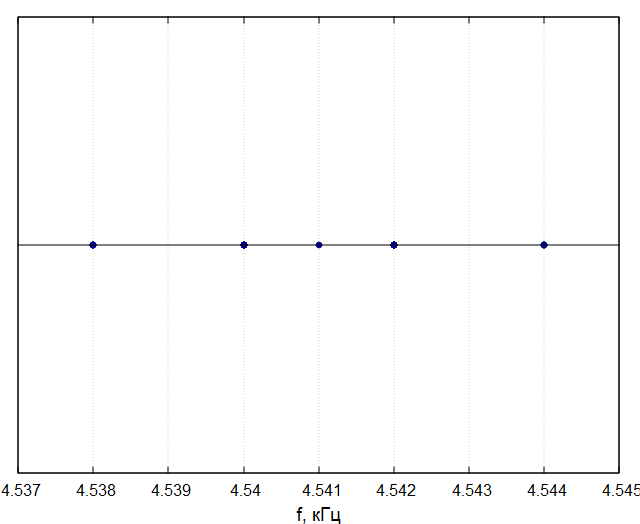
\includegraphics[width=0.8\textwidth]{Plot2.png}
\caption{График распределения результатов наблюдений на числовой оси}
\label{fig:plot2}
\end{figure}

\begin{figure}
\centering
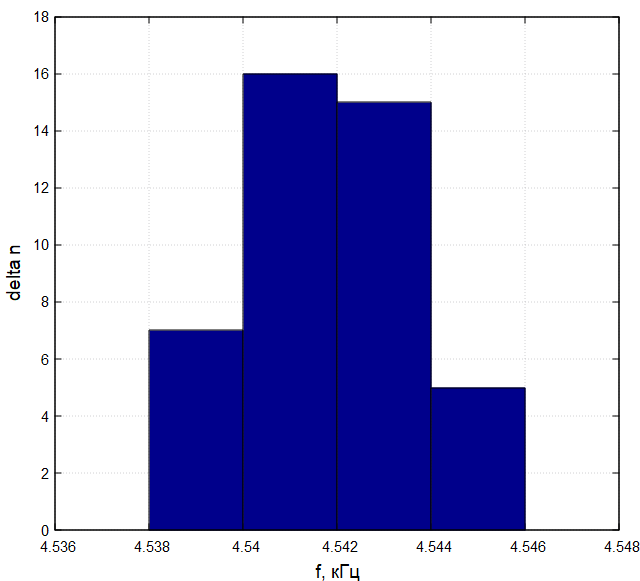
\includegraphics[width=0.75\textwidth]{Plot3.png}
\caption{Гистограмма распределения}
\label{fig:plot3}
\end{figure}

\begin{figure}
\centering
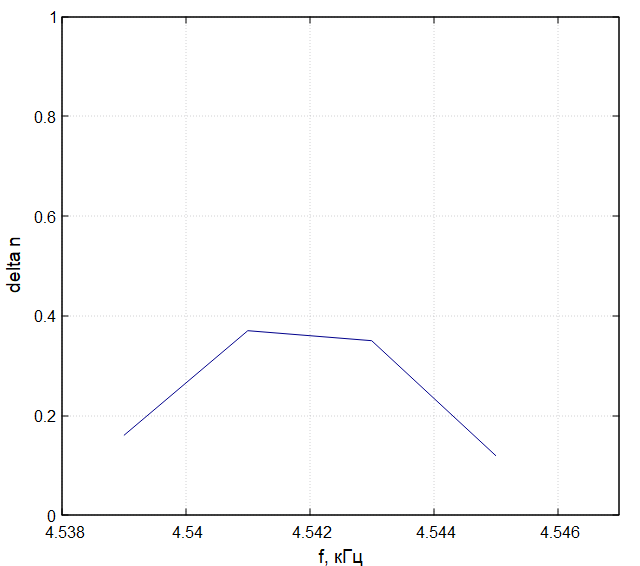
\includegraphics[width=0.74\textwidth]{Plot4.png}
\caption{График зависимости}
\label{fig:plot4}
\end{figure}

\section{Вывод}
Измерения всегда сопровождаются погрешностями, и их анализ играет ключевую роль в обработке экспериментальных данных. Я познакомилась с методикой использования измерительного прибора - частотомера Ч3-32 - для многократных прямых измерений. Научилась основным методам оценки точности, среди которых: вычисление среднего значения, средней квадратичной погрешности, дисперсии, построение гистограммы, графика зависимости. Количество измерений влияет на точность результата: чем больше данных, тем выше надёжность оценки измеряемой величины. Вероятностный анализ позволяет оценить вероятность попадания истинного значения в заданный интервал, что важно для корректного представления результатов измерений. 

\begin{thebibliography}{9}
\bibitem{repo}
\url{https://github.com/st117208/Workshop1}  (дата обращения: 07.03.2025)
\end{thebibliography}